\chapter{仮想記憶}
\label{virtualMemory}
仮想記憶は,物理メモリよりも多くのメモリをプロセスが使用できるようにする.
仮想記憶を実現するために使用できるメモリ管理機構として,
第\ref{chap:segmentation}章で学んだセグメンテーションと,
第\ref{chap:paging}章で学んだページングがある.
既に第\ref{chap:segmentation}章で,
セグメンテーション機構による仮想記憶は簡単に説明した.
しかし,セグメンテーションには,
物理メモリより大きなセグメントを使用できない問題があった.

ページングを用いる方がメリットが多いので,
現代のオペレーティングシステムはページングによる仮想記憶を使用している.
この章ではページングに基づく仮想記憶方式について学ぶ.

%==============================================================================
\section{基本概念}
ページングでは,
ページテーブルのVビットを使用して仮想アドレス空間にフレームが
割り付けられていない状態を表現していた.
Vビットが0のページにアクセスすると
\emph{ページ不在割込み(page fault)}が発生し,
制御がオペレーティングシステムに移る.
Vビットが0の状態を上手く使うことで,
メモリより大きなプログラムでも実行できる仕組みを作る.

\figref{virtualMemoryBasic}に示すように,
ページの内容はフレームかディスク(\emph{バッキングストア})に格納する.
ページの内容がフレームに置かれている時は
ページテーブルの対応するエントリのVビットを1(V=1)にする.
フレームに置かれていない時はV=0とする.
V=0のページにアクセスするとページ不在割込みが発生する.
ページ不在の理由と対処方法は,
例えば以下のようにまとめることができる.

\begin{enumerate}
\item 仮想アドレス空間の無効領域をアクセスし本当にエラーを起こした.\\
  → プロセスを終了する.
\item バッキングストアに内容が退避されているページにアクセスした.\\
  → フレームを割当て内容をディスクから復旧した後,プロセスを再開する.
\end{enumerate}

\begin{myfig}{btp}{仮想記憶の基本}{virtualMemoryBasic}
  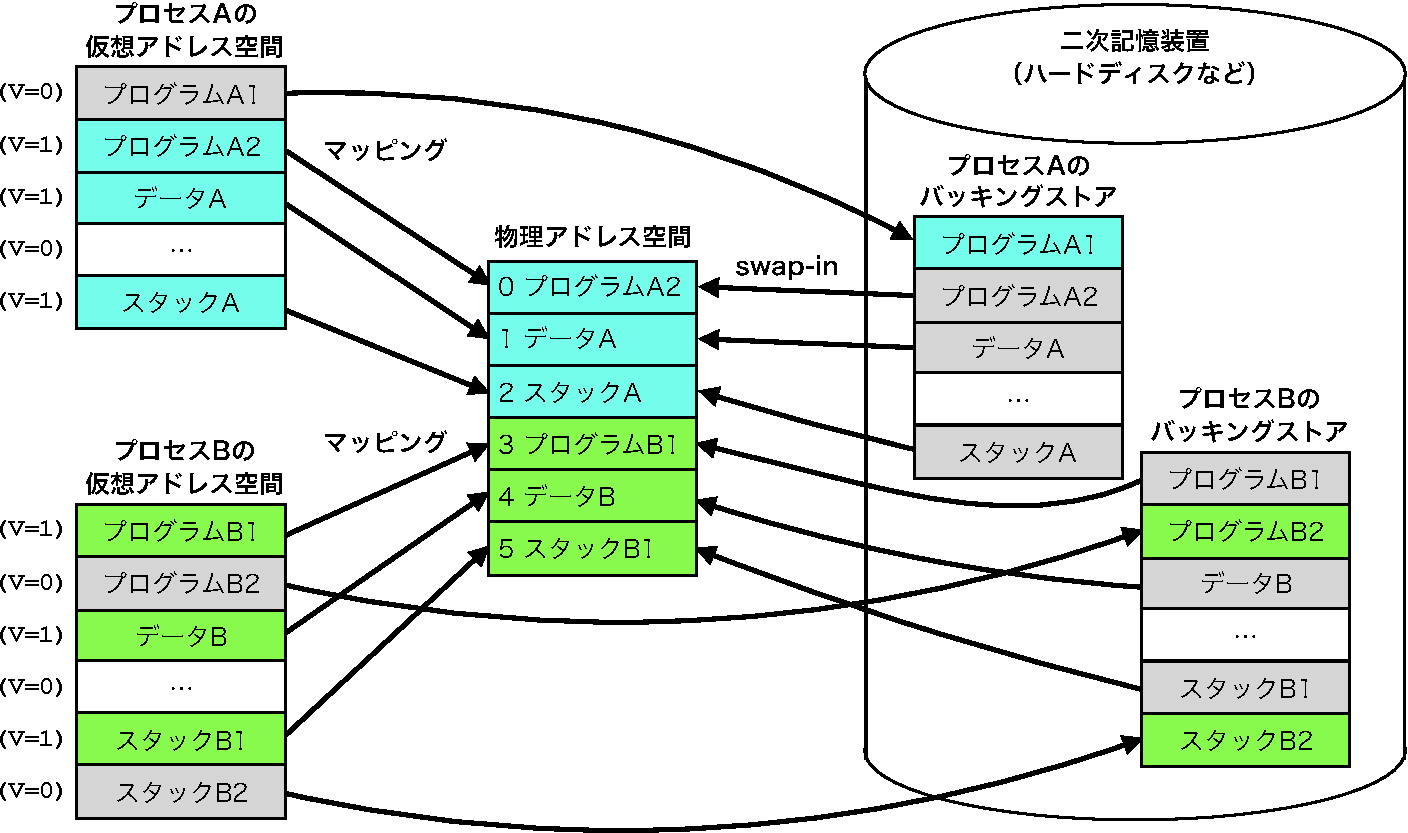
\includegraphics[scale=0.66]{Fig/virtualMemoryBasic-crop.pdf}
\end{myfig}

プロセス生成時にバッキングストアに仮想アドレス空間のイメージを作成する.
フレームは,まだ割当てない.
プログラムが動作を開始するとページ不在割込みが発生し,
その都度,必要なページをバッキングストアから読み込む.

%==============================================================================
\section{デマンドページング}\label{demandPaging}
ページングよる仮想記憶を用いると,
プロセス実行開始時にプログラム全体をメモリに読み込まなくても良い.
原理上は,一ページも読み込まなくても実行を開始することができる.
プログラムの最初の命令をフェッチする時点でページ不在割込みが発生し,
オペレーティングシステムによりページが読み込まれる.
このような,プログラムがアクセスした時点で
ページを読み込む方式を\emph{デマンドページング(Demand Paging)}と呼ぶ.
使用しないページをメモリに読み込むことがない点で無駄がない.
現代の多くのオペレーティングシステムは,
デマンドページング\footnote{デマンドページングの改良版も含む.}を
ページ読み込み方式として採用している.

\subsection{デマンドページングの手順}
デマンドページングの手順を以下にまとめる.

\begin{enumerate}
\item プロセスがV=0のページをアクセスする.
\item ページ不在割込みが発生しオペレーティングシステムに制御が移る.
\item オペレーティングシステムはプロセスがアクセスしたアドレスが
  正当なアドレスか調べる.\\
  不正なアドレスならプロセスを終了させる.(処理終わり)
\item 空きフレームを捜す.\\
  空きフレームが無い場合は何れかのフレームを選択し
  バッキングストアに書き出し(swap-out)空きフレームを作る.
\item 空きフレームをプロセスに割当て
  バッキングストアからページの内容を読み込む(swap-in).
\item ページテーブ等を新しい状態に更新する.
\item ページ不在割込みを発生した命令の再実行からプロセスを再開する.
\end{enumerate}

\subsection{プログラムファイルの直接swap-inによる実行}
プログラムの機械語部分は変更されないので,
swap-out用のバッキングストアを準備する必要はない.
プログラムはデマンドページング方式で実行形式ファイルから直接swap-inする.
バッキングストアに予めプログラムをコピーしたり,
プログラムを予めフレームに読み込んだりしないので,
プログラムの起動を素早く行うことができる.
このアイデアを\figref{virtualMemoryWithZMagic}を用いて説明する.

\begin{myfig}{btp}{デマンドページング}{virtualMemoryWithZMagic}
  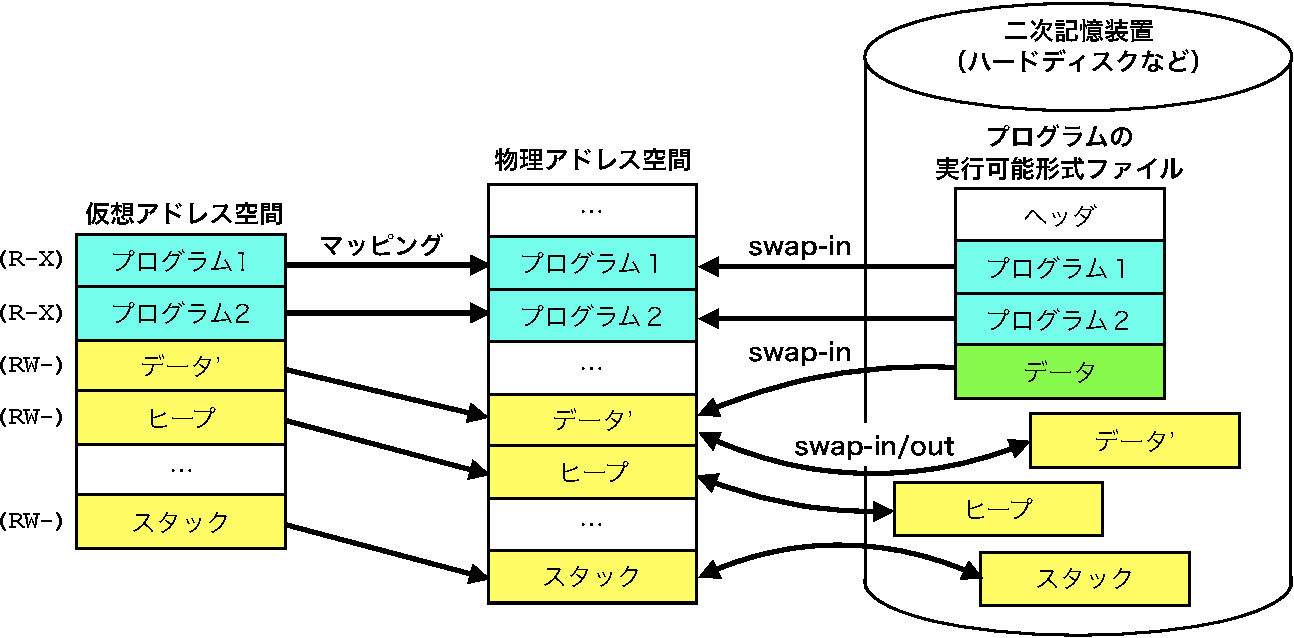
\includegraphics[scale=0.66]{Fig/virtualMemoryWithZMagic-crop.pdf}
\end{myfig}

\begin{enumerate}
\item \emph{実行可能形式ファイルの構造} \\
  プログラムはデマンドページング用の実行可能形式ファイルに格納される.
  このファイルではデマンドページングで使用しやすいように,
  ページサイズの整数倍の境界からセグメントが配置されている.
  \begin{itemize}
  \item ヘッダはファイルがデマンドページング用の実行形式ファイルで
    あることを示すマジックナンバーで始まり,
    ファイル内のセグメントの大きさなどを記述している.
    ヘッダのサイズはページサイズと同じである.
  \item ヘッダの次に,機械語プログラムを格納したセグメントが配置される.
    セグメントの大きさはページサイズの整数倍である.
    \figref{virtualMemoryWithZMagic}は
    プログラムのサイズが二ページの場合である.
  \item プログラムの次に初期化データが配置される.
    初期化データは初期値を明示したグローバル変数を集めた領域である.
  \end{itemize}
\item \emph{プログラムの読み込み} \\
  仮想アドレス空間の\emph{「プログラム1」}ページがアクセスされ
  ページ不在割込みが発生する.
  オペレーティングシステムがフレームを割り付け,
  実行可能形式ファイルから\emph{「プログラム1」}領域をswap-inする.
  プログラム領域は読み出し実行(R-X)だけが許可され,
  値が書き換えられることはない.
\item \emph{初期化データの読み込み} \\
  仮想アドレス空間の\emph{「データ」}ページがアクセスされ,
  ページ不在割込みが発生する.
  オペレーティングシステムがフレームを割り付け,
  実行可能形式ファイルから\emph{「データ」}領域をswap-inする.
  データ領域は読み書き(RW-)が許可されるので値が変化する.
\item \emph{非初期化データとヒープ領域の割り付け} \\
  非初期化データ領域とヒープ領域は連続しているので,
  ここではヒープ領域としてまとめて説明する.
  仮想アドレス空間の\emph{「ヒープ」}ページがアクセスされ
  ページ不在割込みが発生する.
  オペレーティングシステムがフレームを割り付け内容をゼロでクリアする\footnote{
  C言語等の非初期化グローバル変数の初期値がゼロだと保証される.}.
  ヒープ領域は読み書き(RW-)が許可されるので値が変化する.
\item \emph{スタック領域の割り付け} \\
  仮想アドレス空間の\emph{「スタック」}ページがアクセスされ,
  ページ不在割込みが発生する.
  オペレーティングシステムがフレームを割り付け,
  内容をゼロでクリアする\footnote{
  以前フレームを使用したプロセスの機密情報が漏洩しないようにクリアする.}.
  スタック領域は読み書き(RW-)が許可されるので値が変化する.
\end{enumerate}

\subsection{プログラムのswap-out}
プログラムを実行するに従い,
デマンドページングにより,
新しいページが次々とフレームに読み込まれる.
他のプロセスも同じように振る舞うので,やがてフレームが枯渇する.
使用頻度の低いフレームを解放し,再利用できるようにする必要がある.
フレームを解放する際に内容をswap-outする場合がある.
以下では実行中のプロセスの,
各領域のフレームを解放する手順を簡単に述べる.

\begin{enumerate}
\item \emph{プログラム領域} \\
機械語プログラムは読み出し実行(R-X)だけ許可されたページに格納されるので,
swap-inされてから書き換わることはない.
再度ページが必要になった時は,
実行可能形式ファイルから読み込めば良いので,
解放するフレームの内容をswap-outする必要はない.
バッキングストア領域とI/Oトラフィックを小さくすることができる.

\item \emph{初期化データ領域} \\
初期化データ領域は,初期値が格納された状態でswap-inされる.
読み書き可能(RW-)なのでプログラム実行中に書き換わる可能性がある.
ページテーブルのD(Dirty)ビットが0の場合は
読み込み時点から変更されていないのでswap-outする必要はない.
必要になったとき実行可能形式ファイルから読み出し直せば良い.
ページテーブルのD(Dirty)ビットが1の場合は,
フレームを再利用する前にバッキングストアにswap-outし,
次回必要になった時に復元できるようにする.

\item \emph{非初期化データ・ヒープ・スタック} \\
これらの領域は,ゼロで初期化されてから使用が開始される.
読み書き可能(RW-)なのでプログラム実行中に書き換わる可能性がある.
ページテーブルのD(Dirty)ビットが0の場合は
初期化時点から変更されていないので,
何もしないでフレームを解放しても良い.
ページテーブルのD(Dirty)ビットが1の場合は,
フレームを再利用する前にバッキングストアにswap-outし,
次回必要になった時に復元できるようにする.
\end{enumerate}

%==============================================================================
\section{Copy on Write}
UNIXのforkシステムコールはプロセスのコピー(子プロセス)を作る.
多くの場合,
子プロセスはすぐにexecveシステムコールを発行し新しい
プログラムの実行を開始するので,
せっかくコピーした仮想アドレス空間はあまり活用されないまま廃棄される.
これでは効率が悪いのでアドレス空間を親子で共有するvforkシステムコールが
提供されるようになった.
vforkシステコールを用いる場合,
子プロセスがexecveするまで親プロセスは待ち状態になり,
共有のアドレス空間を破壊し合わないような工夫がされた.
その後,\emph{Copy on Write}と呼ばれるアドレス空間のコピーを遅らせる
技術が用いられるようになり,
forkシステムコールを用いても無駄なメモリコピーが起こらなくなった.

\begin{description}
\item[fork直後の様子]
  Copy on Write を用いる場合,
  \figref{virtualMemoryFork}に示すように
  fork直後は親子プロセスでフレームを共有する.
  この時点ではメモリのコピーはしない.
  その代わり,
  書き込み可能であるはずのデータ,ヒープ,スタック領域の
  メモリ保護を読み出し専用に設定する.
  \begin{myfig}{btp}{fork直後の親子プロセス}{virtualMemoryFork}
    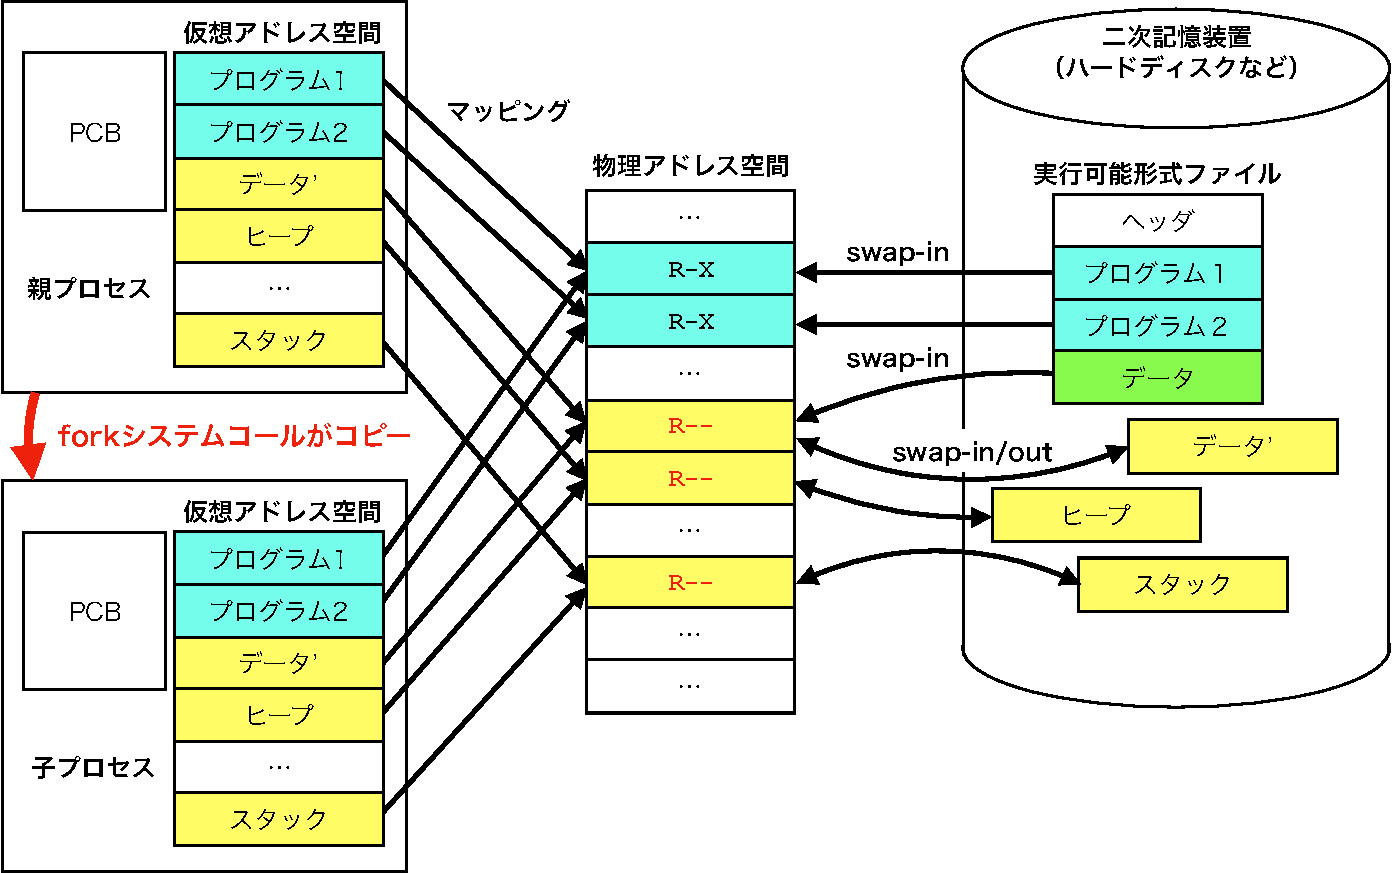
\includegraphics[scale=0.66]{Fig/virtualMemoryFork-crop.pdf}
  \end{myfig}
\item[Copy on Writeの手順]
  どちらかのプロセスがスタックを書き換えようとした場合を例に,
  Copy on Write が働く手順を説明する.
  プロセスがスタック領域を書き換えようとすると
  メモリ保護割込みが発生しオペレーティングシステムに切り換わる.
  その後,オペレーティングシステムが次に述べる操作を行い,
  \figref{virtualMemoryCOW}に示す状態になる.
  \begin{enumerate}
  \item 新しいフレームを割当て,スタック領域フレームの内容をコピーする.
  \item 片方のプロセスのスタック領域に新しいフレームをマッピングする.
    もう一方のプロセスのスタック領域は古いフレームをマッピングしたままにする.
  \item 両プロセスのスタック領域の保護情報を読み書き(RW-)に変更する.
  \item 割込みを発生した命令の再実行からプロセスを再開する.
  \end{enumerate}
  \begin{myfig}{btp}
    {スタックでCopy on Writeが発生した時の親子プロセス}{virtualMemoryCOW}
    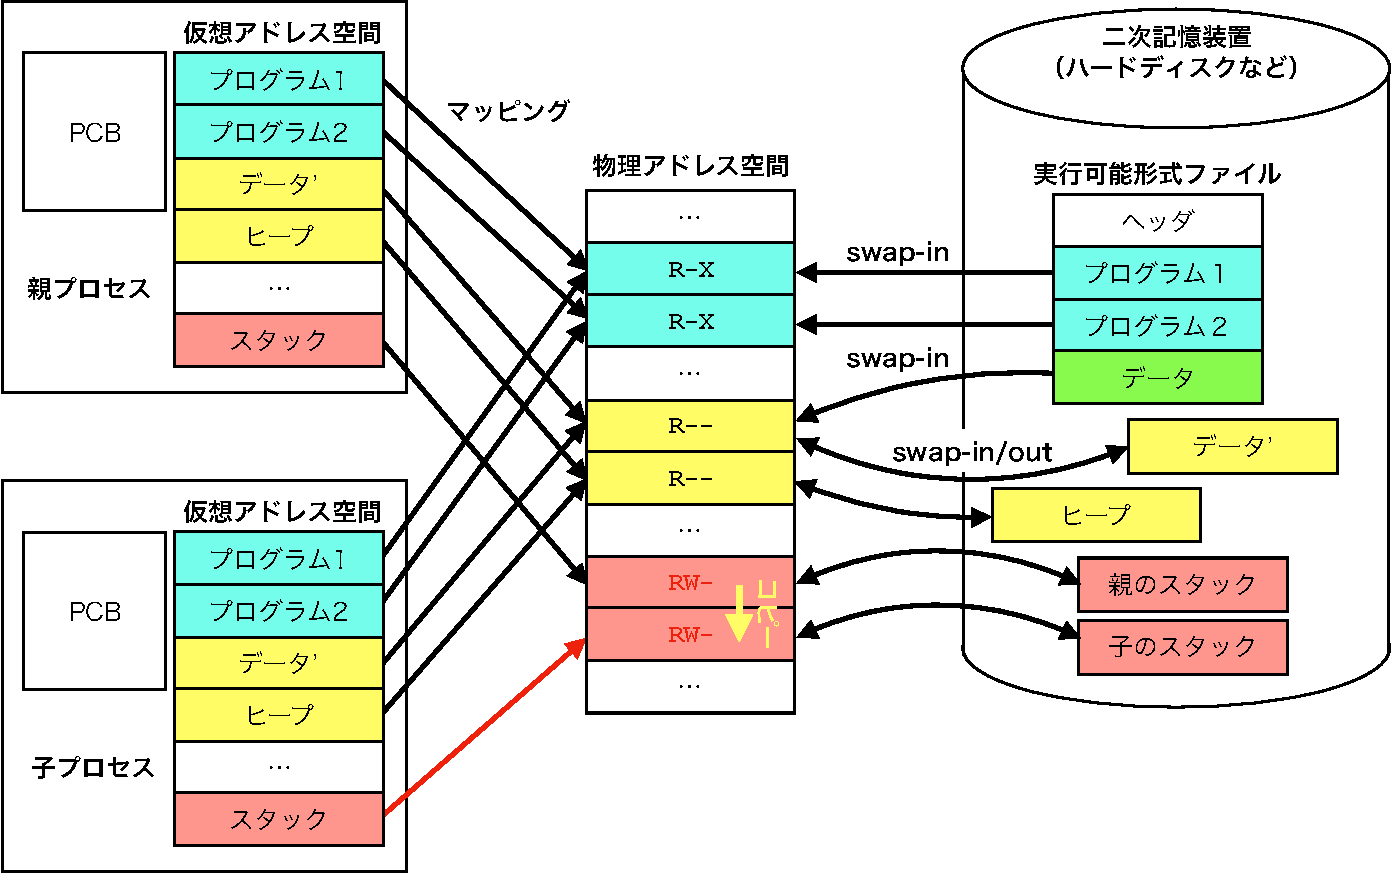
\includegraphics[scale=0.66]{Fig/virtualMemoryCOW-crop.pdf}
  \end{myfig}
\end{description}

以上のように書き込みが起こった時点でメモリがコピーされるので
Copy on Write と呼ばれる.

%==============================================================================
\section{メモリマップドファイル}
仮想記憶機構を用いてファイルを読み書きする手段を提供する.
仮想アドレス空間にファイルをマッピングすることで,
ユーザプログラムがメモリ(配列)を操作する手順でファイルを読み書きできる.
ファイル操作の度にシステムコールを発行しない軽いファイル操作手段である.
また,複数のプロセスが同じファイルをマッピングすることで,
プロセス間の広帯域のデータ共有手段にもなる.

\subsection{UNIXのメモリマップドファイル}
メモリマップドファイルの使用例を示す.
UNIXではmmapシステムコール\footnote{
Windowsでは\texttt{CreateFileMapping()}関数をが使用できる.} を用いて
仮想アドレス空間とファイルを関連付ける.
ファイルを仮想アドレス空間上の配列としてアクセスすることができる.
以下に,mmapシステムコールのプロトタイプ宣言と簡単な解説を掲載する.

\begin{lstlisting}[numbers=none]
void * mmap(void *addr, size_t len, int prot, int flags, int fd, off_t offset);
\end{lstlisting}

\begin{description}
\item[\emph{戻り値}:]
  マップされた領域の先頭アドレスが返される.
  アドレスはページサイズの倍数になる.
\item[\texttt{addr}:]
  マップしたい仮想アドレス空間の先頭アドレスを渡す.
\item[\texttt{len}:]
  マップする領域の大きさを渡す.
  大きさはページサイズの倍数にする.
\item[\texttt{prot}:]
  保護モード(protection)を表す値を渡す.
  ページの保護モード(RWX)が決まる.
\item[\texttt{flags}:]
  ファイルをマップする(\|MAP_FILE|)か
  ファイルに関係づけない名無しメモリをマップする(\|MAP_ANON|)か,
  変更をプロセス間で共用する(\|MAP_SHARED|)か
  プロセスにプライベートにする(\|MAP_PRIVATE|)か等を表すフラグを渡す.
\item[\texttt{fd}:]
  オープン済みファイルのファイルディスクリプタを渡す.
\item[\texttt{offset}:]
  ファイルの\texttt{offset}バイトから始まる
  \texttt{len}バイトをマッピングする.
  \texttt{offset}はページサイズの倍数にする.
\end{description}

リスト\ref{mmapTest}に
ファイルの内容を配列のように書き換えるプログラムの例を掲載する.
このプログラムを実行すると予め作成しておいた\texttt{a.txt}ファイルの
最初の4KiBが英大文字で上書きされる.

\lstinputlisting[numbers=left,float=btp,
  caption=メモリマップドファイルの使用例,label=mmapTest]{Lst/mmapTest.c}

\begin{description}
\item[8行] 予め作成しておいた4KiBのファイルを開く.
  プロセスがメモリマップを通してファイルに読み書き両方ができるためには,
  openシステムコールのフラグに\|O_RDWR|を渡す必要がる.
\item[13行] 仮想アドレス空間に8行でオープンしたファイルをマッピングする.
  マッピングするアドレスの決定をカーネルに任せるので第1引数は\|NULL|にする.
  ファイルをマッピングし書き込んだ内容を反映するために,
  \|MAP_FILE|フラグと\|MAP_SHARED|フラグを指定する.
\item[18行] mmapシステムコールが完了したらファイルはクローズして構わない.
\item[19〜21行] mmapが返した領域を文字型の配列と見做して文字を書き込む. 
  値をファイルに反映するために特別な操作をする必要はない.
\end{description}

\subsection{メモリマップドファイルの仕組み}
\figref{virtualMemoryWithMmap}に,
二つのプロセスの仮想アドレス空間に
同じファイルの同じ部分をマップした例を示す.
UNIXのmmapシステムコールで\|MAP_FILE|フラグと
\|MAP_SHARED|フラグを使用した場合に相当する.
この例では,
ファイルは読み書きの両方ができるようにマップされている.
二つのプロセスは同じフレームを共用し,
共有メモリを持った状態でもある.

\begin{myfig}{btp}
  {プロセス間で共有したメモリマップドファイル}{virtualMemoryWithMmap}
  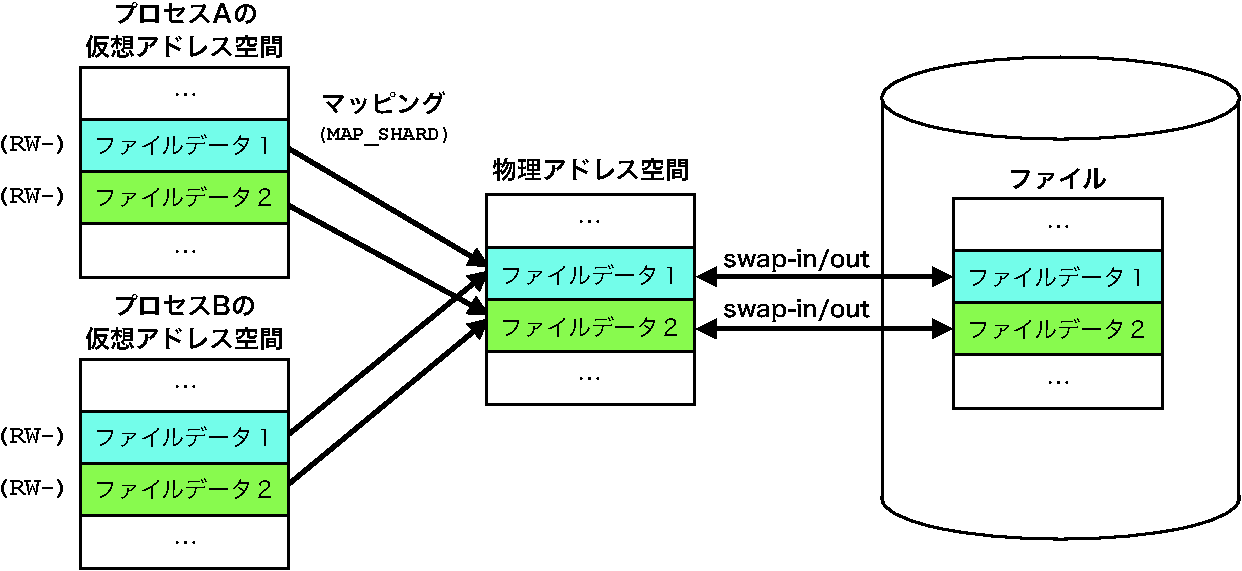
\includegraphics[scale=0.66]{Fig/virtualMemoryWithMmap-crop.pdf}
\end{myfig}

\figref{virtualMemoryWithMmap}は,
ファイルの内容がフレームに読み込まれた状態を表している.
しかし,mmapシステムコール実行直後は,図とは異なり,
フレームが割当てられていない.
mmapはページとファイルを関連付けるが,
実際にファイルを読み書きするのは仮想記憶の仕組みによる.
以下に,メモリマップドファイルが読み書きされる仕組みを説明する.

\begin{enumerate}
\item \emph{ファイルの読み込み} \\
  マップされたアドレスをプロセスがアクセスした時点で,
  ファイルの該当箇所がデマンドページングの要領でフレームに読み込まれる.
\item \emph{ファイルの書き込み} \\
  定期的に変更のあった(Dirty)ページをファイルに書き戻す.
  また,プロセスが終了したりマッピングが解除された時も
  Dirty なページをファイルに書き戻す.
\end{enumerate}

\subsection{read/writeシステムコールとの比較}
メモリマップドファイルの場合,
フレーム上のデータが参照されたり変更される度に
ファイルの読み書きが起こるわけではなく,
効率の良いファイルの参照が可能である.

一方でread/writeシステムコールの場合は,
ディスクキャッシュを用いて二次記憶装置のアクセス回数を
少なくする工夫がされる.
しかし,read/writeシステムコールの引数として渡されたバッファと
ディスクキャッシュの間でメモリコピーをする必要がある.
\figref{mmapVsReadWrite}に,
read/writeシステムコールを使用する場合のデータの流れを模式的に示す.
メモリコピーは一般に重い処理である.

\begin{myfig}{btp}{read/writeシステムコールのデータコピー}{mmapVsReadWrite}
  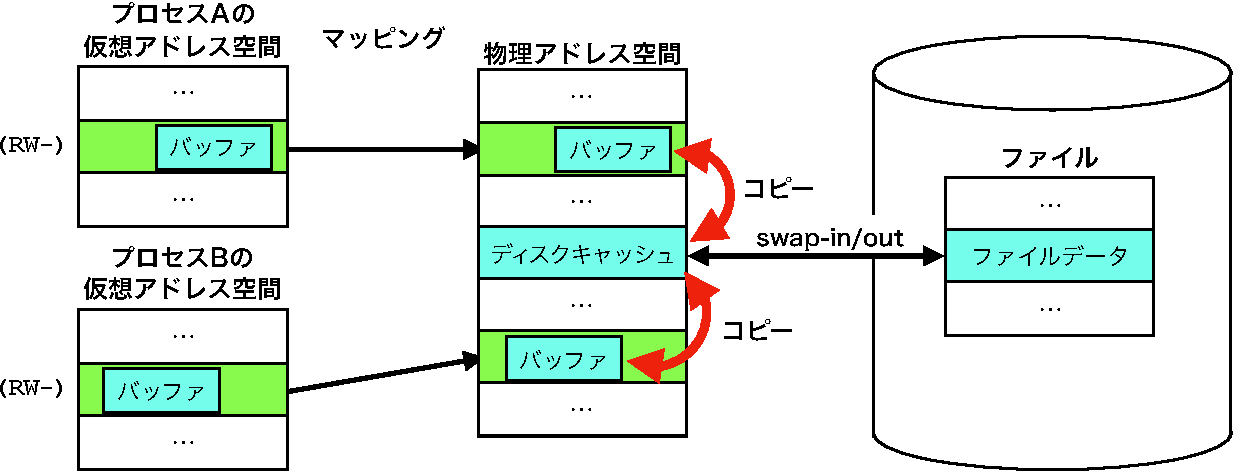
\includegraphics[scale=0.66]{Fig/mmapVsReadWrite-crop.pdf}
\end{myfig}

また,read/writeの場合はデータの読み書きの度にシステムコールを発行する.
一方でメモリマップドファイルの場合,
mmapシステムコールを用いてマッピングを完了してしまえば
システムコールを発行する必要がない.
システムコールも一般に重い処理である.

\subsection{プロセスにローカルなマッピング}
\figref{virtualMemoryWithPrivateMap}に,
二つのプロセスの仮想アドレス空間に
同じファイルの同じ部分を\emph{ローカルに}マップした例を示す.
UNIXのmmapシステムコールで\|MAP_PRIVATE|フラグを使用した場合に相当する.

\begin{itemize}
\item \emph{「ファイルデータ1」}領域 \\
プロセスの仮想アドレス空間にマップされ,かつ,プロセスに参照された.
参照された時点でフレームに読み込まれプロセスから見える状態になっている.
\item \emph{「ファイルデータ2」}領域 \\
一旦,「ファイルデータ1」のように参照されフレームに読み込まれた.
その後,プロセスが値を書き換えた.
\|MAP_PRIVATE|の場合は他のプロセスやファイルに変更が反映されない.
\emph{Copy on Write}方式でコピーが作られ,
プロセス毎に別のコピーが参照されるようにマッピングする.
\end{itemize}

\begin{myfig}{btp}
  {プロセスにローカルなメモリマップドファイル}{virtualMemoryWithPrivateMap}
  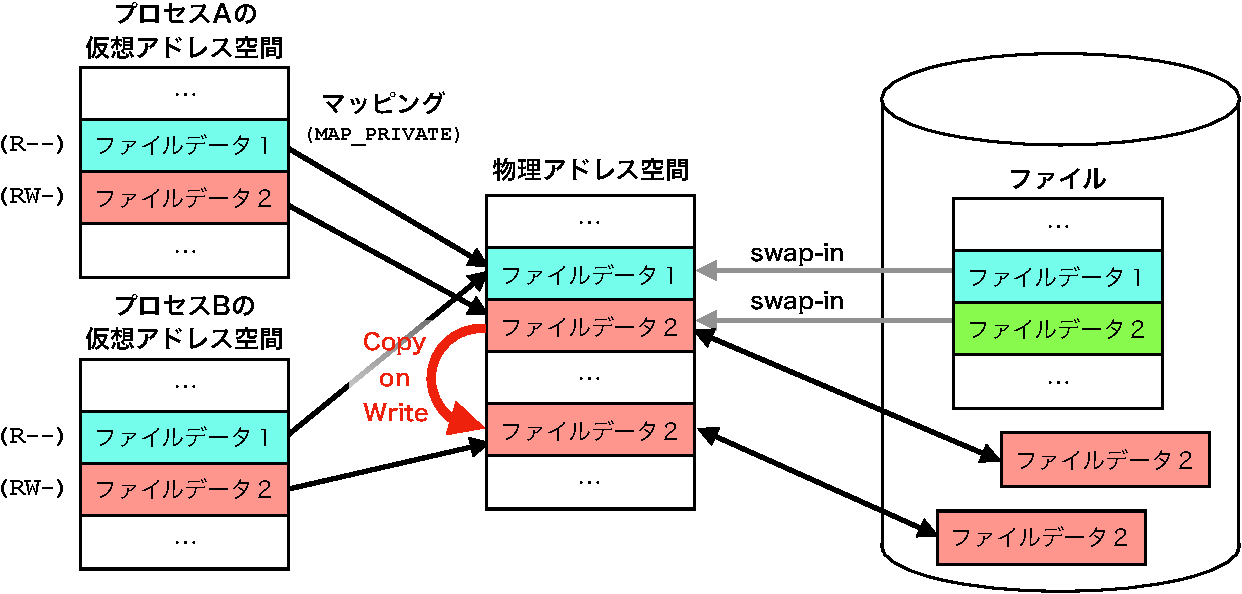
\includegraphics[scale=0.66]{Fig/virtualMemoryWithPrivateMap-crop.pdf}
\end{myfig}

\subsection{無名メモリのマッピング}
\figref{virtualMemoryWithAnonymousMap}に,
\emph{無名メモリ}のマッピング例を示す.
無名メモリはファイルと関連付けられないが,
最初に内容がファイルからロードされるのではなく
\emph{ゼロでクリアされる}ことを除いて・
メモリマップドファイルのプロセスにローカルなマッピングと同様な管理を受ける.
UNIXのmmapシステムコールでは\|MAP_ANON|フラグを使用して無名メモリを割り付ける.

\begin{myfig}{btp}{無名メモリのマッピング例}{virtualMemoryWithAnonymousMap}
  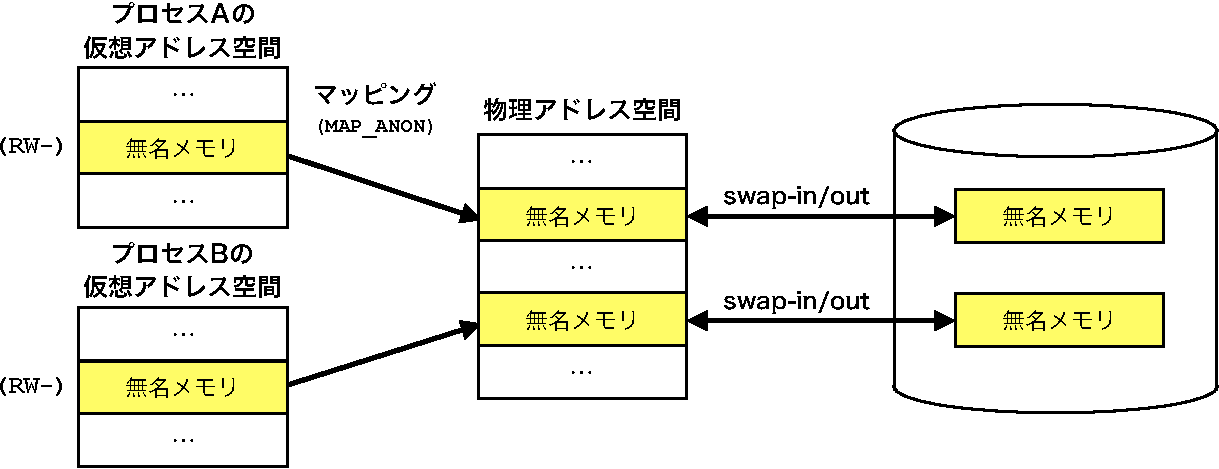
\includegraphics[scale=0.66]{Fig/virtualMemoryWithAnonymousMap-crop.pdf}
\end{myfig}

\subsection{プログラムの実行とメモリマップドファイル}
メモリマップドファイルの仕組みと,
\figref{virtualMemoryWithZMagic}で見た
デマンドページングによるプログラムの実行は,
以下のようにメモリマップドファイルを用いると実現できる.
BSD UNIX では実際にメモリマップドファイルと同じ
仕組みを利用している\cite{execOfFreeBSD}.

\begin{itemize}
\item 実行形式ファイルをメモリにマッピングする.
  \begin{itemize}
  \item プログラムは,\|R-X|でマッピングする\footnote{
    \texttt{R-X}なら\texttt{MAP\_SHARED}でも\texttt{MAP\_PRIVATE}でも同じ.}
    \footnote{
      BSD UNIX では,デバッガがブレークポイントを設定できるように,
      \texttt{RWX},\texttt{MAP\_PRIVATE}でマッピングしている
      \cite{execOfFreeBSD}.}.
         (プログラムはプロセス間で共用される)
  \item 初期化データは,\|RW-|,\|MAP_PRIVATE|でマッピングする.
    書き込みが起きた時点でバッキングストアと結びつける.
  \end{itemize}
\item 非初期化データ,ヒープ,スタックは,
  無名メモリ(\|RW-|,\|MAP_ANNON|)割り当てる.
\end{itemize}

%==============================================================================
\section{ページ置き換えアルゴリズム}
ページングによる仮想記憶では,
以下の三つの重要なアルゴリズムを定める必要がある.

\begin{enumerate}
\item \emph{ページ読み込みアルゴリズム} : いつページをswap-inするか決める.
  \ref{demandPaging}で既に学んだデマンドページングを用いる.
\item \emph{ページ置き換えアルゴリズム} : フレーム不足時に,
  どのページを再利用するか決める.
  本節で学ぶ.
\item \emph{フレーム割り付けアルゴリズム} : どのフレームを使用するか決める.
  \ref{frameAllocation}で学ぶ.
\end{enumerate}

デマンドページングによりページが読み込まれるにつれ,
システムの空きフレームが少なくなっていく.
大量のメモリを使用するプロセスや,
同時に多数のプロセスが実行される状況では,
やがて空きフレームが枯渇してしまう.

更にページを読み込む必要が生じた時,
\emph{どれかのプロセス}の\emph{どれかのページ}を再利用する.
再利用することに決めたページは,
ロードされた後で内容が変更されていればバッキングストアに書き出(swap-out)し,
フレームをプロセスから取り上げる.
このフレームを再利用することで実行を継続する.
\emph{ページ置き換えアルゴリズム}は,どのプロセスの,
どのページを解放するか決めるアルゴリズムである.
将来,使用されないフレームをうまく選択しないと,
swap-outしたページが直後にswap-inされることになり,
システムの性能が著しく低下する.

\subsection{局所性・ワーキングセット・フェーズ化}
プログラムの実行中,
全てのページが均等にアクセスされ続けることは稀である.
普通は一部のページにアクセスが集中し,
また,アクセスが集中するページは時刻によって変化していく.
その様子を\figref{locality}に示す.

\begin{myfig}{btp}{局所性・ワーキングセット・フェーズ化}{locality}
  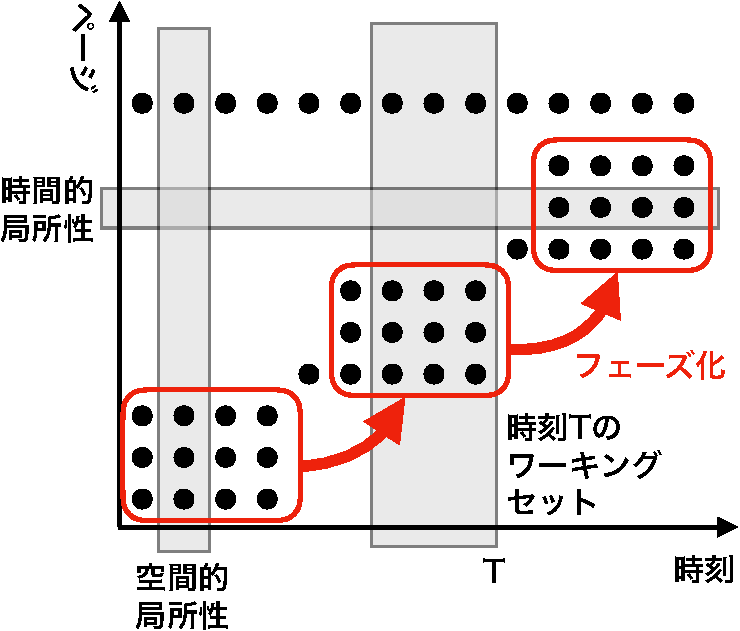
\includegraphics[scale=0.66]{Fig/locality-crop.pdf}
\end{myfig}

\begin{description}
\item[局所性]
  短い時間に着目すると,
  一部の連続したページが集中的にアクセスされる.
  これを\emph{空間的局所性}と呼ぶ.
  また,あるページに着目すると一部の連続した時刻にアクセスが集中している.
  これを\emph{時間的局所性}と呼ぶ.
\item[ワーキングセット]
  プログラム実行中のある時間にアクセスされるページの集合を,
  その時間の\emph{ワーキングセット}と呼ぶ.
  同時に実行するプロセスを増やすとワーキングセットが大きくなる.
  ワーキングセットが利用可能なフレームの集合より大きくなる
  (ワーキングセットがメモリに入り切らなくなる)とページ不在が多発する.
  %新しいページを読み込むための
  swap-in/outが繰り返され多くのプロセスがディスクI/O待ちになり,
  システムの性能が急激に低下する.
  このような状態を\emph{スラッシング}と呼ぶ.
\item[フェーズ化現象]
  プログラム実行中,
  時期によりワーキングセットが急激に変化する現象を\emph{フェーズ化現象}と呼ぶ.
  例えば,
  まず,プログラムはデータを入力する.
  この時点では入力処理を含むページがワーキングセットになる.
  次に,プログラムは入力したデータを使用して計算を行う.
  この時点では計算処理を含むページがワーキングセットになる.
  最後に,プログラムは計算結果を出力する.
  この時点では出力処理を含むページがワーキングセットになる.
  フェーズが遷移する時は局所性が失われ,
  ページ不在が集中的に発生する.
\end{description}

ページ置き換えアルゴリズムは,
プログラムのこれら性質に着目した様々な方式が提案されている.

\subsection{LRU(Least Recentry Used)アルゴリズム}
「最近アクセスされていないページは,この先もアクセスされる可能性が低い」との
仮定に基づく方式である.
時間的局所性をプログラムが持っているなら最良の方式である.
しかし,現実的な実装が困難とされている.
もしも実装するとすると\figref{pagingLRU}のようなハードウェアが必要になる.
CPUはメモリアクセス毎に値がインクリメントされる十分に長いカウンタ\footnote{
64bitのカウンタなら毎秒1Gi回のメモリアクセスがあったとしたとしても,
500年以上オーバーフローしない.
}を備える.
ページテーブルにはカウンタの値を保存できる「最終アクセス時刻」フィールドが
追加されている.

\begin{myfig}{btp}{LRU方式のためのハードウェア}{pagingLRU}
  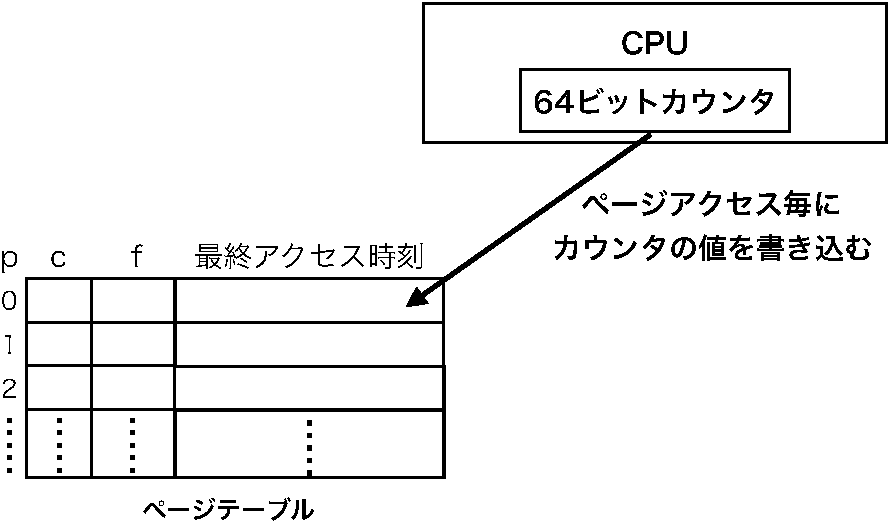
\includegraphics[scale=0.66]{Fig/pagingLRU-crop.pdf}
\end{myfig}

\begin{enumerate}
\item メモリアクセス毎に,
  アクセスしたページのページテーブルエントリにカウンタの値を書き込む.
\item ページ不在が発生し空きフレームが無いなら,
  ページテーブルをスキャンし最も古いページを見つける.
\item 見つけたページをswap-outし,代わりに目的のページをswap-inする.
\end{enumerate}

この方式の問題は,
ハードウェアのコストと,
ページ不在時の処理の重さである.
ページ不在は頻繁に発生する\footnote{
macOSの vm\_stat コマンドを用いると,
毎秒数千回のページ不在が発生する様子を見ることができる.}ので,
その度にページテーブル全体をスキャンすることは現実的ではない.

\subsection{LFU(Least Frequently Used)アルゴリズム}
LRUの近似方式の一種であり,
ページテーブルのRビット(\tabref{pageTableAttr}参照)と,
フレーム毎のカウンタだけを用いてソフトウェアで実現できる.
NFU(Not Frequently Used)とも呼ばれる.
次のようなアルゴリズムである.

\begin{enumerate}
\item ページテーブルのRビットとフレームのカウンタをゼロにクリアする.
\item 定期的(例えばTICK=20ms毎)にページテーブルをスキャンする.
  R=1のエントリを見つけたら対応するフレームのカウンタをインクリメントし,
  Rをゼロにクリアする.
\item ページ不在時にフレームが不足したなら,
  カウンタの値が最小のフレームを置き換える.
\end{enumerate}

この方式の問題点は,
ページ不在時にページテーブルのスキャンが必要なことと,
一度カウンタの値が大きくなったフレームは
使用されなくなっても値が大きいままなので,
置き換えられ難いことである.
この問題を解決するために,
定期的にページテーブルをスキャンする際の
カウンタの更新方法を次のように改良した
\emph{エージングアルゴリズム}が提案された.
この改良により,過去のRビットの影響が徐々に小さくなる.

\begin{description}
\item[R=1のフレーム]
  $cnt \leftarrow cnt \div 2 + 0x8000$(カウンタは16bitと仮定)
\item[R=0のフレーム]
$cnt \leftarrow cnt \div 2$
\end{description}

\subsection{FIFO(First-In First-Out)アルゴリズム}
「長くメモリに滞在しているページは役割を終えている」との仮定に基づく.
特別なハードウェアを用いることなく,ソフトウェアだけで実現できる.
\figref{pagingFIFO}のようなリストを用いるアルゴリズムである.

\begin{myfig}{btp}{FIFOアルゴリズムが用いるリスト}{pagingFIFO}
  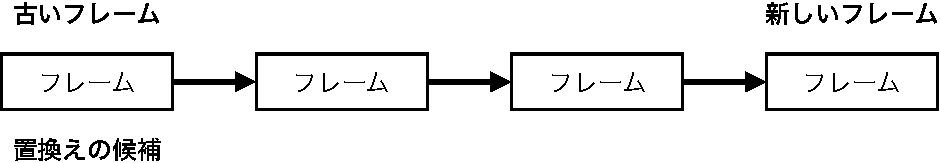
\includegraphics[scale=0.66]{Fig/pagingFIFO-crop.pdf}
\end{myfig}

\begin{enumerate}
\item swap-in する度にフレームをリストの最後(図の右側)に追加していく.
\item ページ不在時にフレームが不足したなら,
  リストの先頭のフレームを置き換える.
\end{enumerate}

このアルゴリズムはページテーブルのスキャンが不要なので非常に軽い.
しかし,常時使用される重要なページも時間が経過するとswap-outされる問題がある.
また,\emph{Beladyの異常な振る舞い}をすることがある.
Beladyの異常な振る舞いとは,
メモリが多い場合の方がページ不在の回数が増える現象である.

\begin{figure}[btp]
  \begin{itembox}[l]{Beladyの異常な振る舞いの例}
    FIFOアルゴリズムを用い,
    ページ参照ストリング(W : 1 2 3 4 1 2 5 1 2 3 4 5)の場合
    \begin{itemize}
    \item フレーム数(m=3)の場合(ページ不在9回)\\
      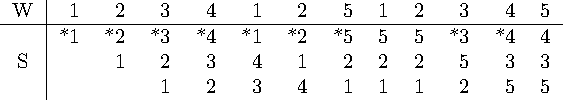
\includegraphics[scale=1.0]{Tbl/beladyAnomalyM3.pdf}
    \item フレーム数(m=4)の場合(ページ不在10回)\\
      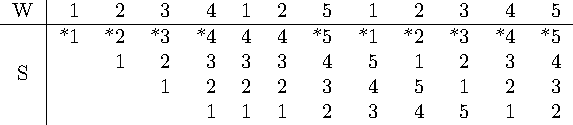
\includegraphics[scale=1.0]{Tbl/beladyAnomalyM4.pdf}
    \end{itemize}
    メモリが多い方(m=4)のページ不在回数が多い.
  \end{itembox}
\end{figure}

\subsection{Clock アルゴリズム}
\figref{pagingClock}に示すようなFIFOのリストを環状にしたデータ構造を用いる.
データ構造に加えてページテーブルのRビットも使用する.
次のようなアルゴリズムである.

\begin{myfig}{btp}{Clockアルゴリズムが用いる環状リスト}{pagingClock}
  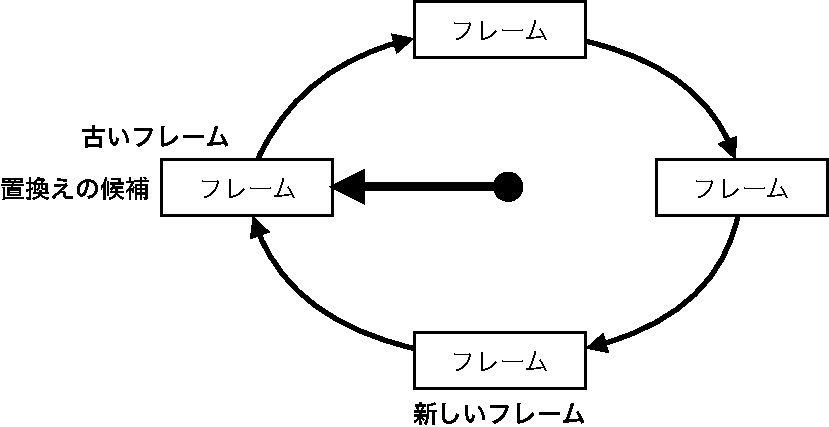
\includegraphics[scale=0.66]{Fig/pagingClock-crop.pdf}
\end{myfig}

\begin{enumerate}
\item swap-inする度にフレームを環状リストに挿入していく.
  挿入位置は最も古いフレームの一つ手前である.
  最も古いフレームは時計の針に当たるポインタが指している.
\item 定期的(例えばTICK=20ms毎)に全ページテーブルエントリのRビットを
  ゼロにクリアする.
\item ページ不在時にフレームが不足したなら,
  時計の針が指しているフレームのページテーブルエントリのRビットを調べる.
  \begin{description}
  \item[R=0の場合]
    ページは古く,かつ,最近アクセスされていないので置き換える.
  \item[R=1の場合]
    ページは古いが最近アクセスされている.
    Rビットをクリアして時計の針を一つ進め,
    次のフレームについて同じ処理を行う.
  \end{description}
  最悪でも時計の針が一周回るとR=0のページが見つかる.
\end{enumerate}

\subsection{WSClock アルゴリズム}
ワーキングセットを考慮したClockアルゴリズムである.
単純でパフォーマンスが良いので,
広く使用されている\cite{wsClock}.
\figref{pagingWSClock}に示すような環状リストを用いる.
リストのノードにはフレームが最近アクセスされた時刻が記録してある.
現在時刻と比較して時刻が古くなっているフレームは,
ワーキングセットから外れたと判断する.
また,ページテーブルのRビットとDビットも使用する.
次のようなアルゴリズムである.

\begin{myfig}{btp}{WSClockアルゴリズムが用いる環状リスト}{pagingWSClock}
  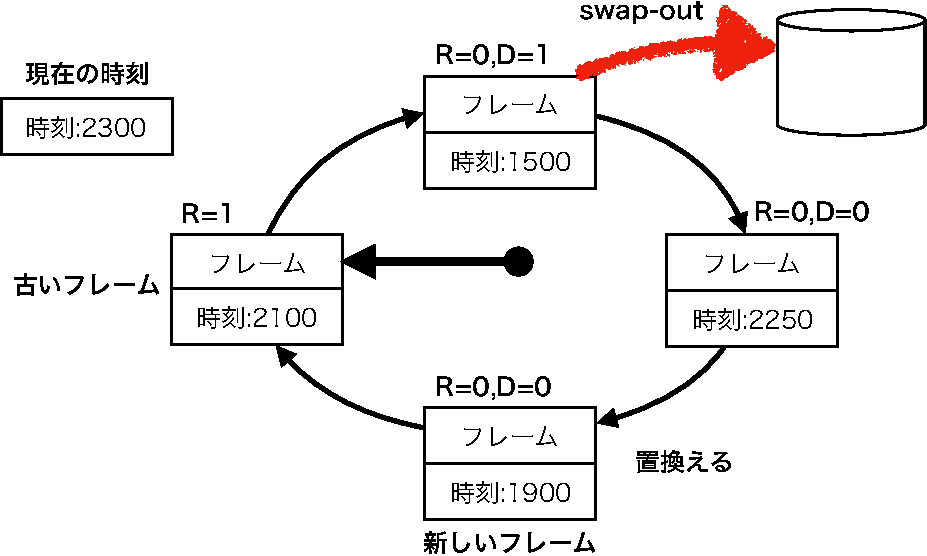
\includegraphics[scale=0.66]{Fig/pagingWSClock-crop.pdf}
\end{myfig}

\begin{enumerate}
\item swap-inする度にフレームを環状リストに挿入していく.
  挿入位置は最も古いフレームの一つ手前である.
  最も古いフレームは時計の針に当たるポインタが指している.
\item 定期的(例えばTICK=20ms毎)に全ページテーブルエントリのRビットを
  ゼロにクリアする.
  その際,R=1だったフレームだけに現在時刻を記録する.
\item ページ不在時にフレームが不足したなら,
  時計の針が指しているフレームを調べる.
  \begin{description}
  \item[R=1の場合]
    Rビットをクリアして次のフレームに進む.
  \item[時刻が新しい場合]
    ページはワーキングセットに含まれている.
    次のフレームに進む.
  \item[時刻が古い場合]
    ページはワーキングセットに含まれていない.
    \begin{description}
      \item[D=1の場合]
        内容が変更されているのでswap-outを予約し,次のフレームに進む.
      \item[D=0の場合]
        このフレームを置き換える.
    \end{description}
  \end{description}
\end{enumerate}

%==============================================================================
\section{フレーム割り付けアルゴリズム}\label{frameAllocation}
ページングシステムでは全てのフレームが同等なので,
どのフレームを,どのプロセスの,どのページに使用しても良い.
任意の空きフレームを使用すれば良いのでフレーム割り付けは問題にならない.
CPUが複数ある場合でも,
\figref{hardBlock}のようなSMPシステムであれば全てのフレームが均質である.

しかし,\figref{intelServer}に示したサーバ用のSMPシステムでは
事情が少し異なっている.
このようなシステムは,
CPUとメモリからなる\emph{ノード}が相互接続された構造になっている.
CPUと異なるノードのメモリは,
CPUと同じノードのメモリより低速なアクセスしかできない.
そこで可能な限り,
同じプロセスのフレームは同じノードのメモリを使用し,
かつ,
同じプロセスのスレッドは同じノードのCPUが実行するようにする.

%==============================================================================
\section{まとめ}
本章ではページングに基づく仮想記憶を学んだ.
ページング機構では,ページテーブルのVビットを用いて
フレームが割り当てられいないページを表現できた.
V=0のページがアクセスされると\emph{ページ不在割込み(page fault)}が
発生するので,その時点で内容を\emph{バッキングストア}から\emph{swap-in}する.
一方で利用頻度の低いページは\emph{swap-out}する.
この手法でメモリより大きなプログラムを実行可能にする.

データをコピーする際,
複数のプロセスがフレームを共有する状態を作った後,
ページに書込みがあった時点でフレームをコピーし
プロセス夫々が異なる内容を持つことを可能にする.
このように,書込みがある時点でコピーを行う方式を\emph{Copy on Write}と呼ぶ.

\emph{メモリマップドファイル}は,
仮想アドレス空間にファイルをマッピングすることで,
ファイルを読み書きする手段を提供する.
本章ではメモリマップドファイルを使用するUNIXプログラムの例を示した.
メモリマップドファイルを用いると,
マッピング完了後はシステムコールを使用することなくファイルの内容を変更できる.

フレームが不足した際に,
swap-out するページを選択するアルゴリズムを
\emph{ページ置き換えアルゴリズム}と呼ぶ.
プログラム実行中のページ参照に\emph{局所性}があり,
\emph{ワーキングセット}の変化により\emph{フェーズ化現象}が生じる.
ワーキングセットがメモリに入り切らないと\emph{スラッシング}が発生する.
ページ置き換えアルゴリズムはこれらの性質を考慮して決定される.
\emph{LRUアルゴリズム},\emph{LFUアルゴリズム},\emph{FIFOアルゴリズム},
\emph{Clokアルゴリズム},\emph{WSClockアルゴリズム}を紹介した.

%==============================================================================
\section*{練習問題}
\begin{enumerate}
  \renewcommand{\labelenumi}{\ttfamily\arabic{chapter}.\arabic{enumi}}
  \setlength{\leftskip}{1em}
\item 次の言葉の意味を説明しなさい.
  \begin{itemize}
  \item 仮想記憶
  \item バッキングストア
  \item ページ不在割込み(page fault)
  \item デマンドページング(demand paging)
  \item swap-in,swap-out
  \item Copy on Write
  \item メモリマップドファイル
  \item 局所性
  \item ワーキングセット
  \item フェーズ化
  \item スラッシング
  \item ページ読み込みアルゴリズム
  \item ページ置き換えアルゴリズム
  \item フレーム割り付けアルゴリズム
  \item LRU,LFU,FIFO,Clock,WSClockアルゴリズム
  \item Beladyの異常な振る舞い
  \end{itemize}
\item リスト\ref{mmapTest}のプログラムを実際に実行してみなさい.
\item 「Beladyの異常な振る舞いの例」で示した
  ページ参照ストリングとフレーム数を用い,
  LRU,LFU,FIFO,Clockアルゴリズムを適用した場合をトレースしなさい.
\end{enumerate}
